\section{Frequency mode 19}
\label{sec:fm19}

\subsection{Overview}
\label{sec:fm19:overview}
Frequency mode~19 monitors the band $556.598$--$557.398\,\mathrm{GHz}$. Its
main use is retrievals of \chem{H_2O} and \chem{O_3}.

\TODO{General text about FM19}
\TODO{Show spectra?}

\subsection{Comparison of retrieved profiles}
\label{sec:fm19:comparison}


%%%%%%
% O3 %
%%%%%%

\subsubsection{\chem{O_3}}
\label{sec:fm19:comparison:O3}
The retrievals for \chem{O_3} have been compared with data from the MIPAS, MLS,
OSIRIS and SAGE~III instruments. Annual average differences to these
instruments are shown in Figure~\ref{fig:fm19:O3:profiles}. In
Figure~\ref{fig:fm19:O3:scatter} individual retrievals for the instruments for
the entire period are plotted against the retrievals from the new and old
versions of the \smr\ processing chain. The results show a better over-all
correlation with the updated version of the processing compared to SAGE~III and
OSIRIS, but worse correlation with MIPAS and MLS, and a systematic under
estimation of the concentrations remains compared to all considered
instruments.
\TODO{reference Fig.~\ref{fig:fm19:O3:mr_avk} in text!}

\begin{figure}[htpb]
    \centering
    \begin{subfigure}[b]{0.49\textwidth}
        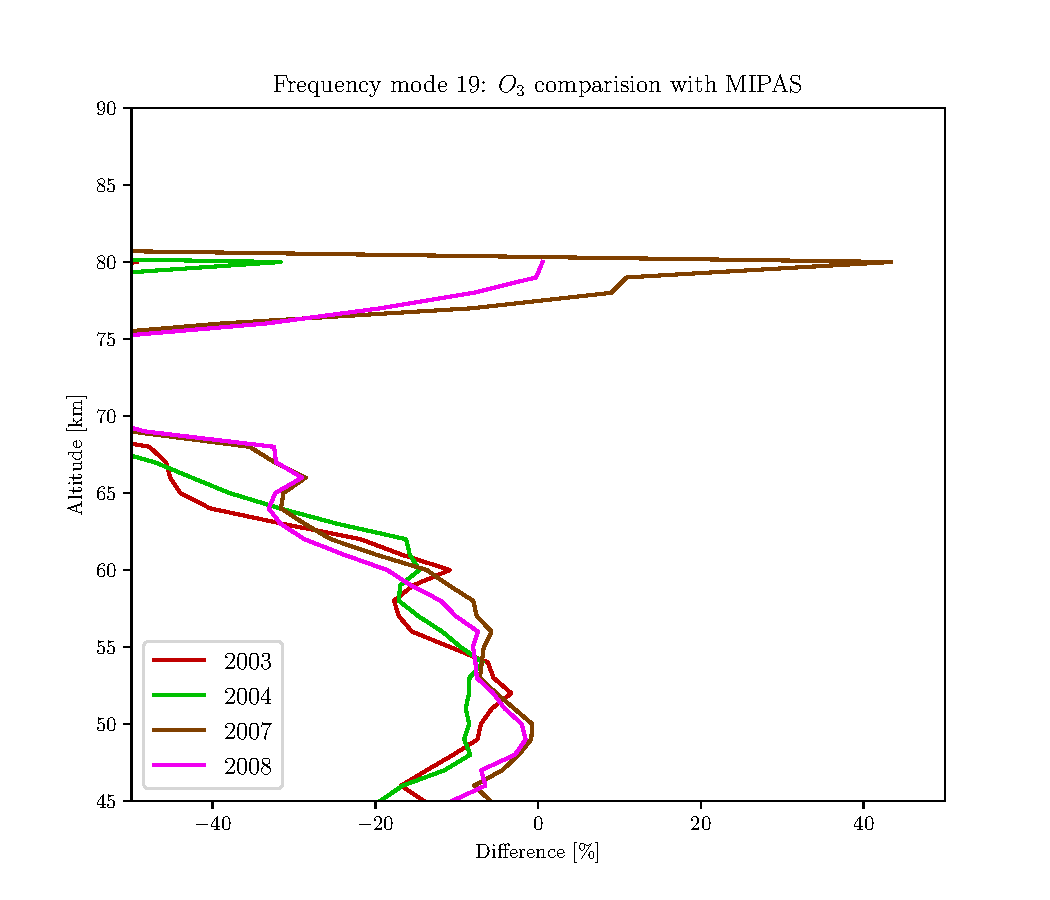
\includegraphics[width=\textwidth]{DDS_fm19_O3_perdiff_mipas}
        \caption{average difference to MIPAS}
        \label{fig:fm19:O3:profiles:MIPAS}
    \end{subfigure}
    \,
    \begin{subfigure}[b]{0.49\textwidth}
        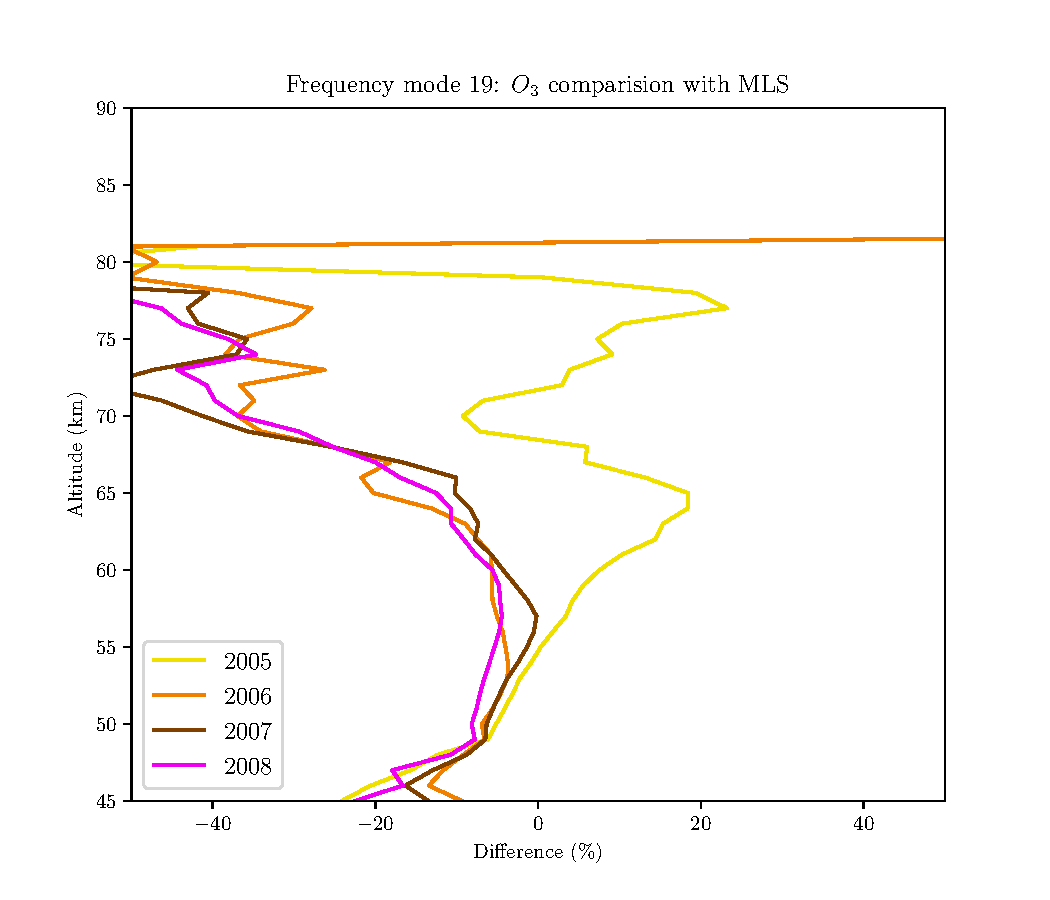
\includegraphics[width=\textwidth]{DDS_fm19_O3_perdiff_mls}
        \caption{average difference to MLS}
        \label{fig:fm19:O3:profiles:MLS}
    \end{subfigure}

    \begin{subfigure}[b]{0.49\textwidth}
        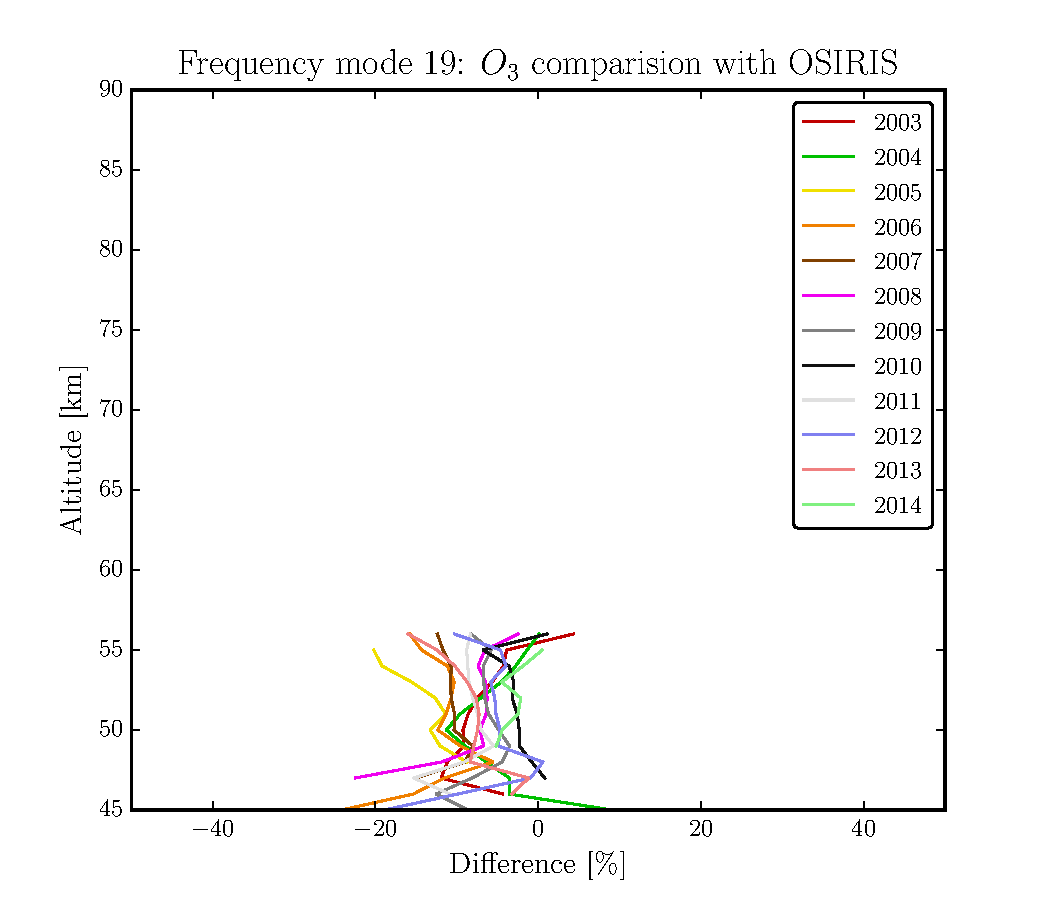
\includegraphics[width=\textwidth]{DDS_fm19_O3_perdiff_osiris}
        \caption{average difference to OSIRIS}
        \label{fig:fm19:O3:profiles:OSIRIS}
    \end{subfigure}
    \,
    \begin{subfigure}[b]{0.49\textwidth}
        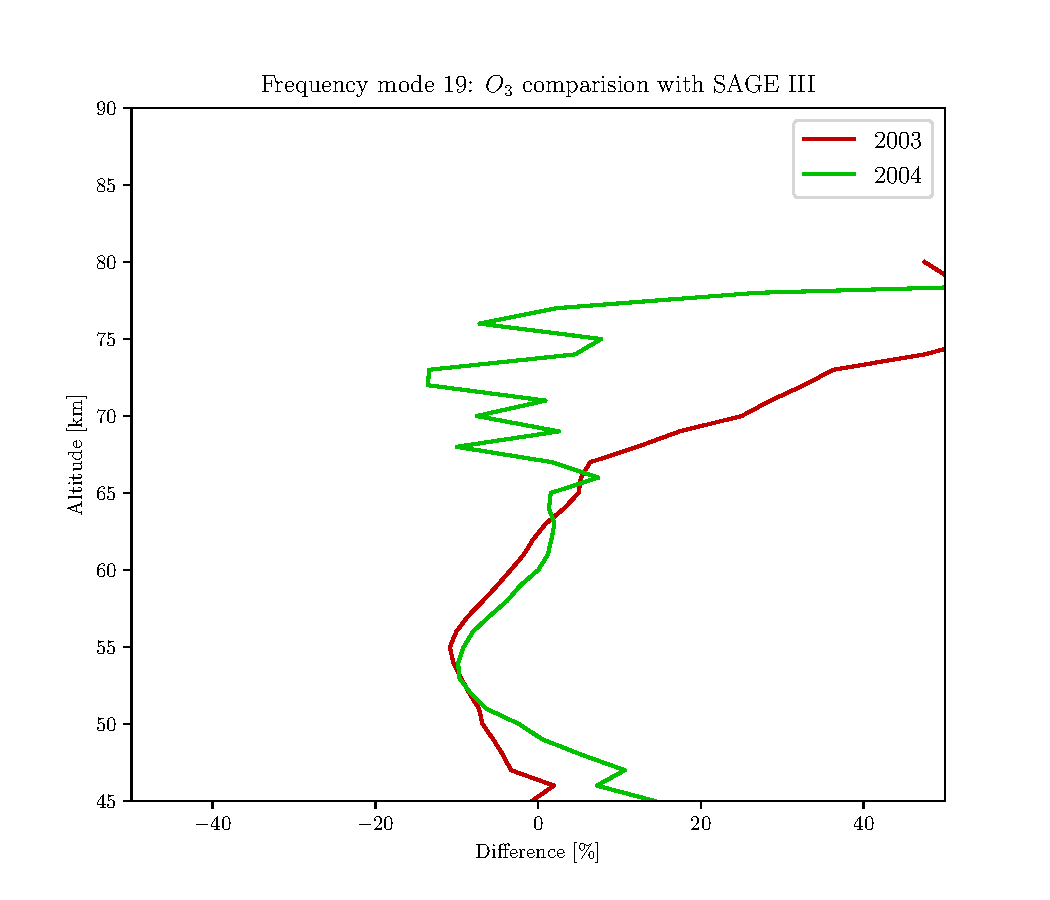
\includegraphics[width=\textwidth]{DDS_fm19_O3_perdiff_sage}
        \caption{average difference to SAGE~III}
        \label{fig:fm19:O3:profiles:SAGEIII}
    \end{subfigure}
    \caption{Average difference in percent between retrievals of \chem{O_3}
    from \smr~v3 and collocated measurements from various instruments at
    different altitudes for frequency mode~19.}

    \label{fig:fm19:O3:profiles}
\end{figure}

\begin{figure}[htpb]
    \centering
    \begin{subfigure}[b]{0.49\textwidth}
        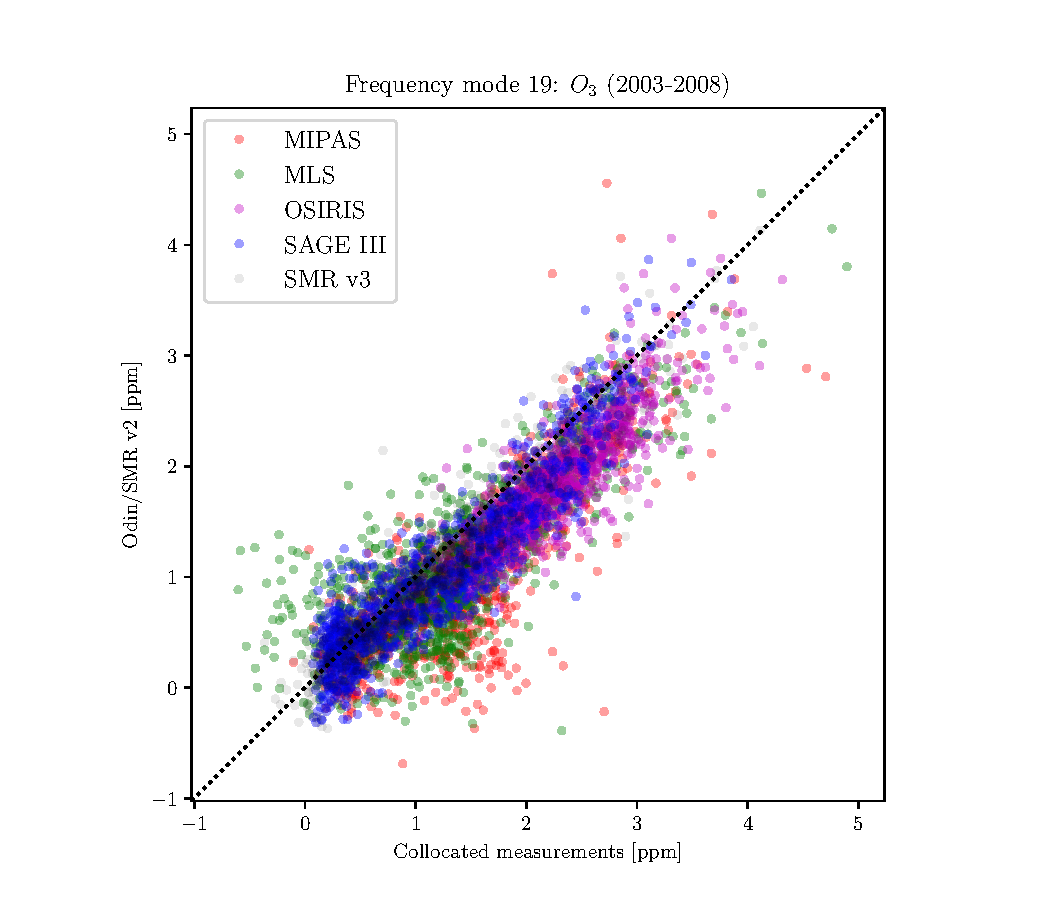
\includegraphics[width=\textwidth]{DDS_fm19_O3_scatter_v2}
        \caption{correlation of collcated instruments with \smr~v2.X}
        \label{fig:fm19:O3:scatter:v2}
    \end{subfigure}
    \,
    \begin{subfigure}[b]{0.49\textwidth}
        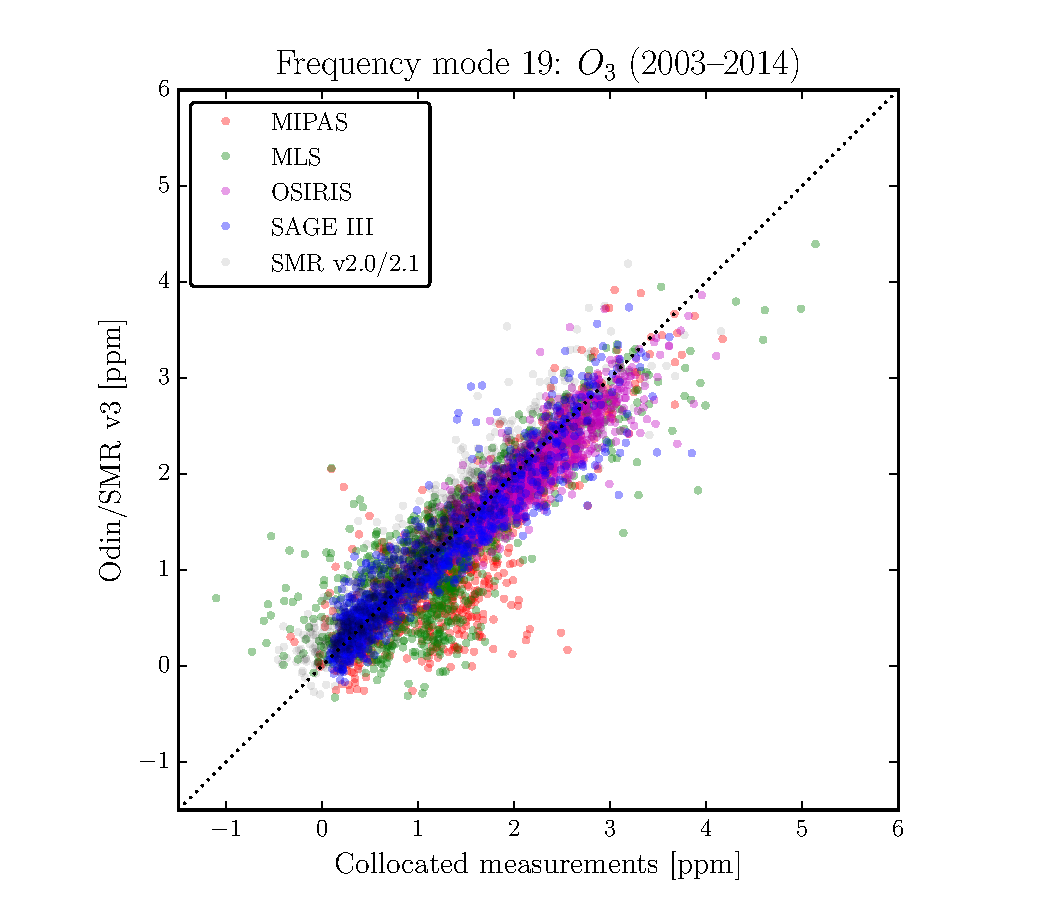
\includegraphics[width=\textwidth]{DDS_fm19_O3_scatter_v3}
        \caption{correlation of collcated instruments with \smr~v3}
        \label{fig:fm19:O3:scatter:v3}
    \end{subfigure}
    \caption{Correlation between retrievals of \chem{O_3} using \smr\
    versions~2.X and~3 and collocated measurements from various instruments
    for frequency mode~19.}
    \label{fig:fm19:O3:scatter}
\end{figure}

\begin{figure}[htpb]
    \centering
    \begin{subfigure}[b]{0.49\textwidth}
        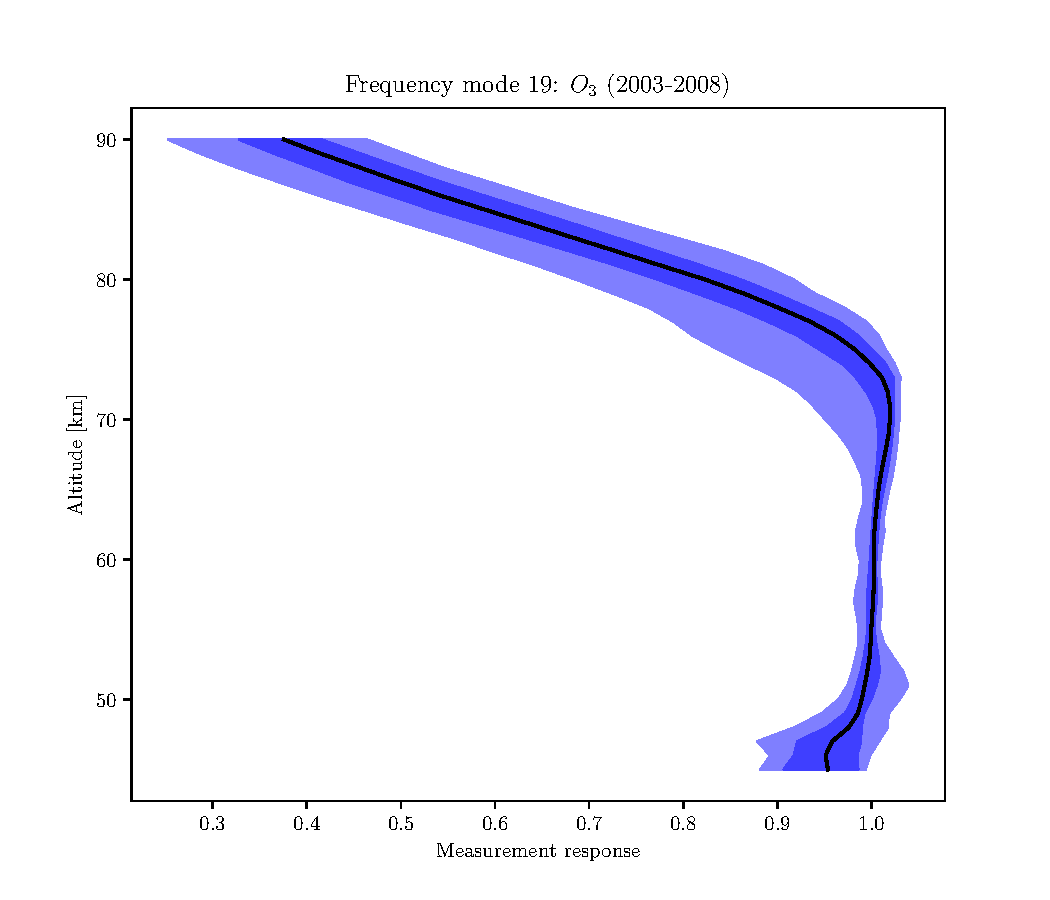
\includegraphics[width=\textwidth]{DDS_fm19_O3_mr}
        \caption{median measurement response with $1\sigma$ and $2\sigma$
        percentiles}
        \label{fig:fm19:O3:mr}
    \end{subfigure}
    \,
    \begin{subfigure}[b]{0.49\textwidth}
        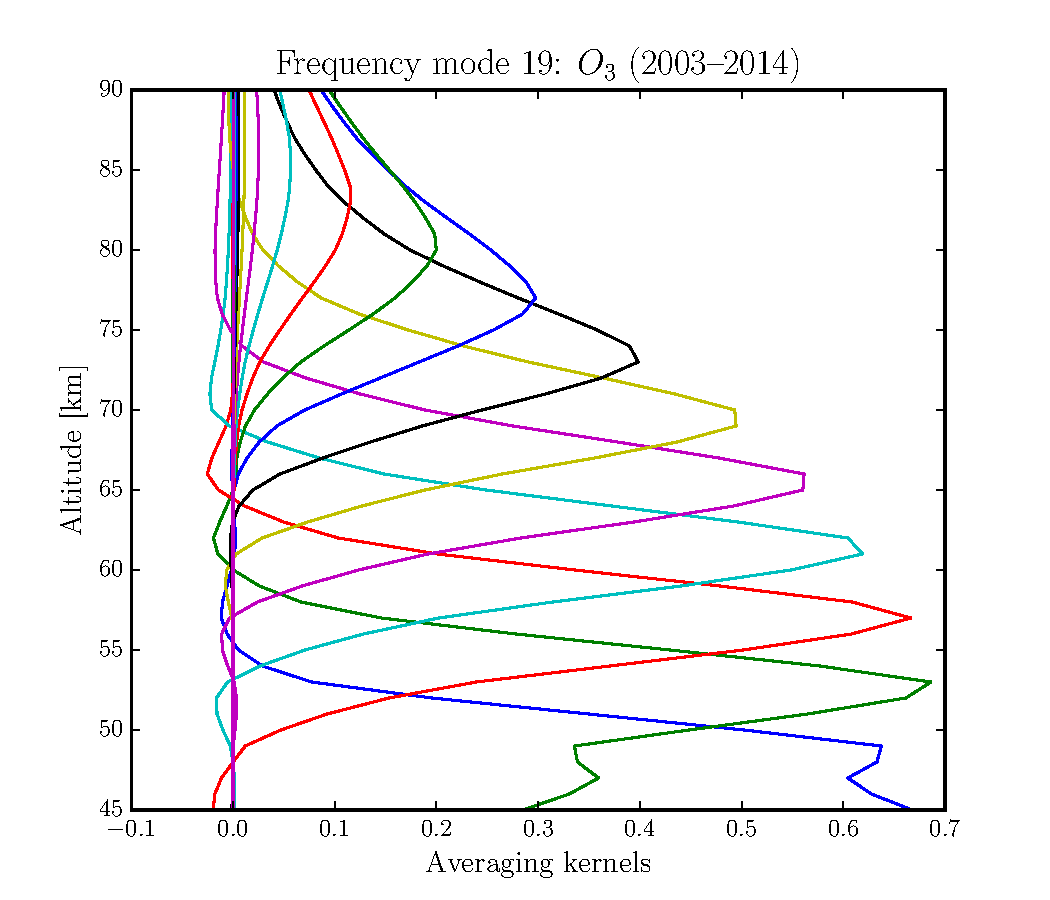
\includegraphics[width=\textwidth]{DDS_fm19_O3_avk}
        \caption{median averaging kernels\newline~}
        \label{fig:fm19:O3:avk}
    \end{subfigure}
    \caption{Measurement response and averaging kernels for \chem{O_3}
    retrievals for \smr~v3 at different altitudes for frequency mode~19.}
    \label{fig:fm19:O3:mr_avk}
\end{figure}


%%%%%%%
% H2O %
%%%%%%%

\subsubsection{\chem{H_2O}}
\label{sec:fm19:comparison:H2O}
The retrievals for \chem{H_2O} have been compared with data from the MIPAS and
MLS instruments.  Annual average differences to these instruments are shown in
Figure~\ref{fig:fm19:H2O:profiles}. In Figure~\ref{fig:fm19:H2O:scatter}
individual retrievals for the instruments for the entire period are plotted
against the retrievals from the new and old versions of the \smr\ processing
chain. The results show a lightly improved over-all correlation with the
updated version of the processing compared to both considered instruments, but
a systematic under estimation of the concentrations has been introduced, and
the correlation with both instruments remains poor.

The SAGE~III instrument also measures \chem{H_2O}, but the there are too few
collocated measurements wit frequency mode~19 for a relevant analysis.
\TODO{reference Fig.~\ref{fig:fm19:H2O:mr_avk} in text!}

\begin{figure}[htpb]
    \centering
    \begin{subfigure}[b]{0.49\textwidth}
        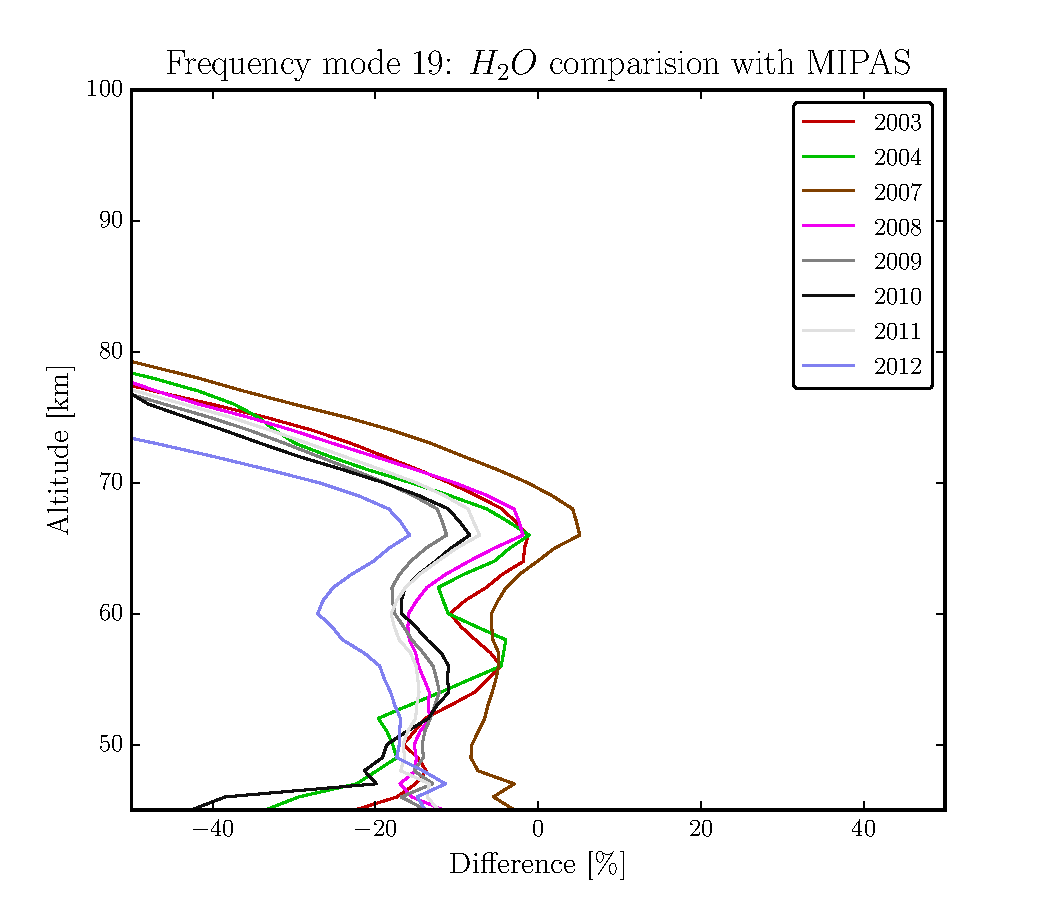
\includegraphics[width=\textwidth]{DDS_fm19_H2O_perdiff_mipas}
        \caption{average difference to MIPAS}
        \label{fig:fm19:H2O:profiles:MIPAS}
    \end{subfigure}
    \,
    \begin{subfigure}[b]{0.49\textwidth}
        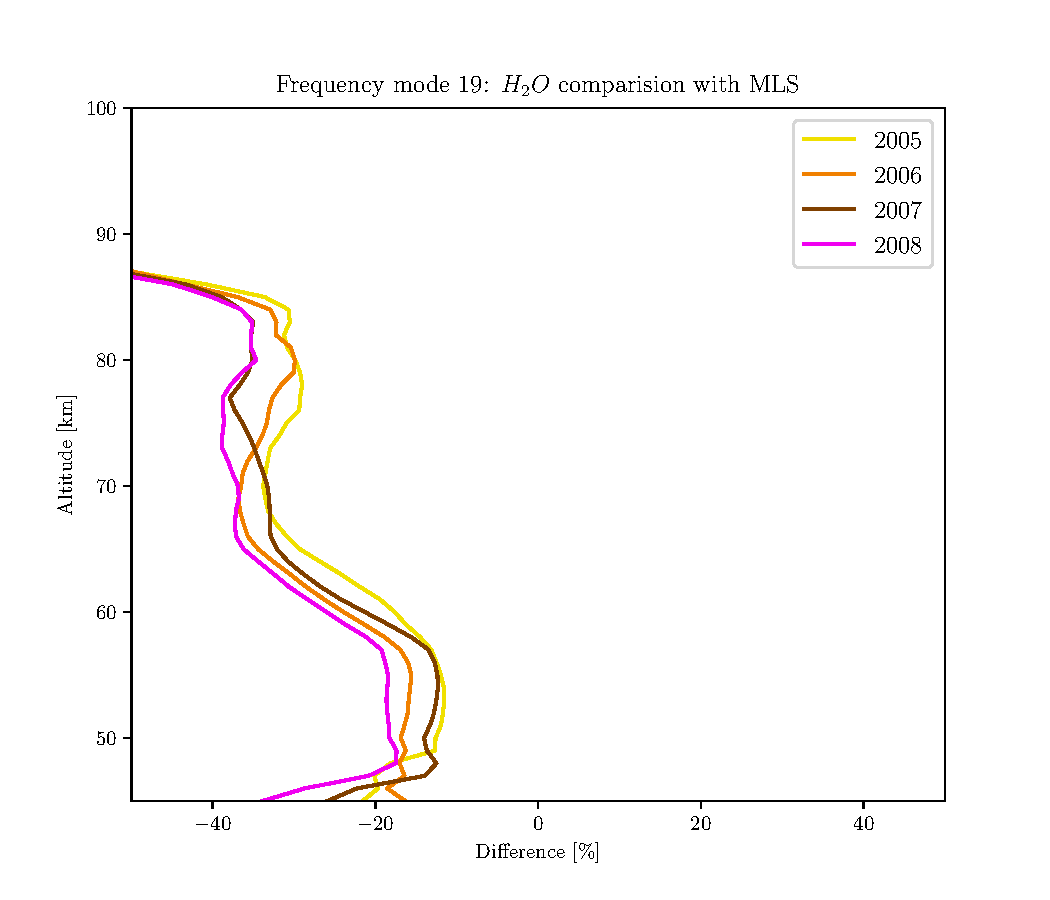
\includegraphics[width=\textwidth]{DDS_fm19_H2O_perdiff_mls}
        \caption{average difference to MLS}
        \label{fig:fm19:H2O:profiles:MLS}
    \end{subfigure}
    \caption{Average difference in percent between retrievals of \chem{H_2O}
    from \smr~v3 and collocated measurements from various instruments at
    different altitudes for frequency mode~19.}

    \label{fig:fm19:H2O:profiles}
\end{figure}

\begin{figure}[htpb]
    \centering
    \begin{subfigure}[b]{0.49\textwidth}
        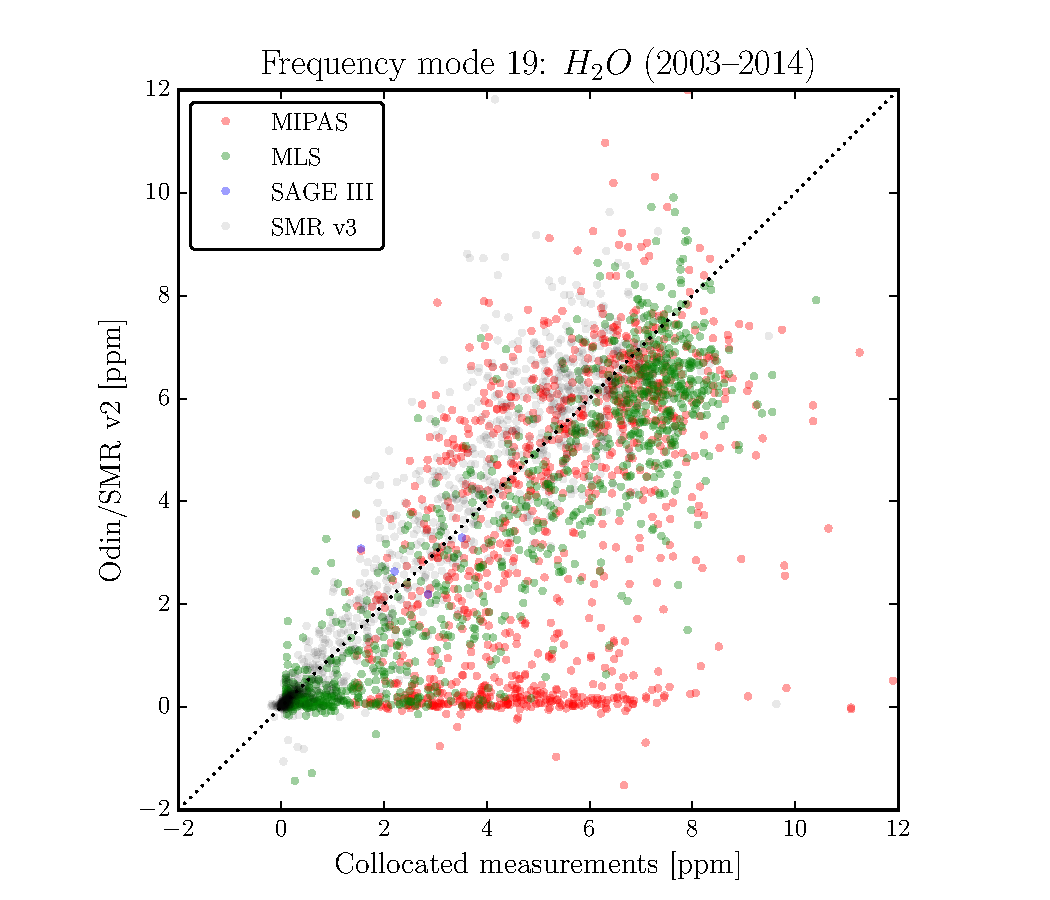
\includegraphics[width=\textwidth]{DDS_fm19_H2O_scatter_v2}
        \caption{correlation of collcated instruments with \smr~v2.X}
        \label{fig:fm19:H2O:scatter:v2}
    \end{subfigure}
    \,
    \begin{subfigure}[b]{0.49\textwidth}
        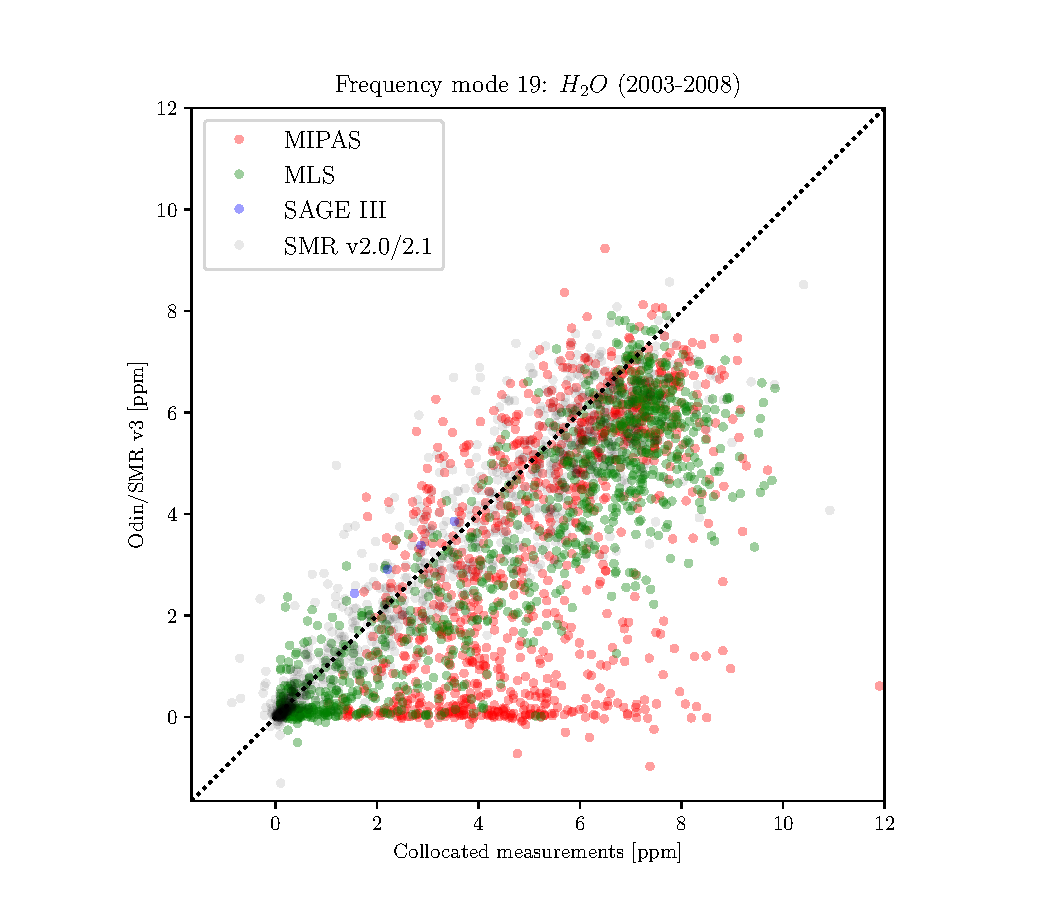
\includegraphics[width=\textwidth]{DDS_fm19_H2O_scatter_v3}
        \caption{correlation of collcated instruments with \smr~v3}
        \label{fig:fm19:H2O:scatter:v3}
    \end{subfigure}
    \caption{Correlation between retrievals of \chem{H_2O} using \smr\
    versions~2.X and~3 and collocated measurements from various instruments
    for frequency mode~19.}
    \label{fig:fm19:H2O:scatter}
\end{figure}

\begin{figure}[htpb]
    \centering
    \begin{subfigure}[b]{0.49\textwidth}
        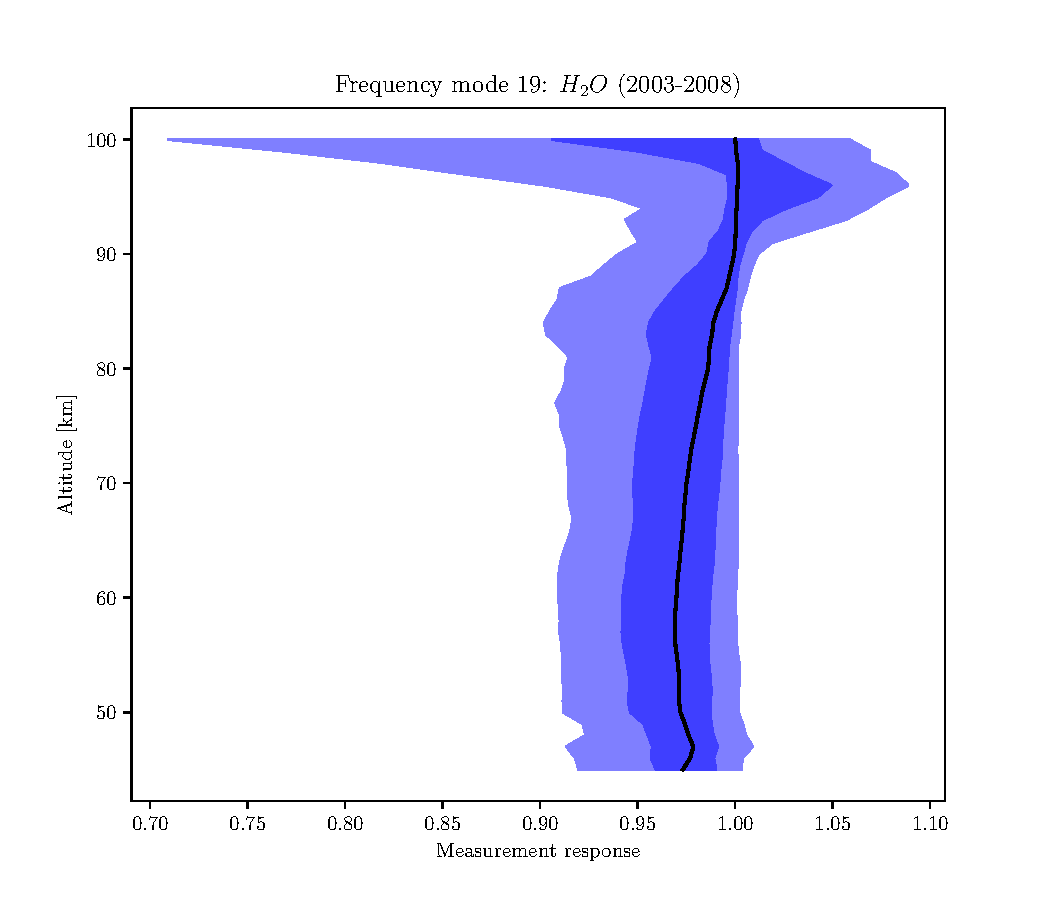
\includegraphics[width=\textwidth]{DDS_fm19_H2O_mr}
        \caption{median measurement response with $1\sigma$ and $2\sigma$
        percentiles}
        \label{fig:fm19:H2O:mr}
    \end{subfigure}
    \,
    \begin{subfigure}[b]{0.49\textwidth}
        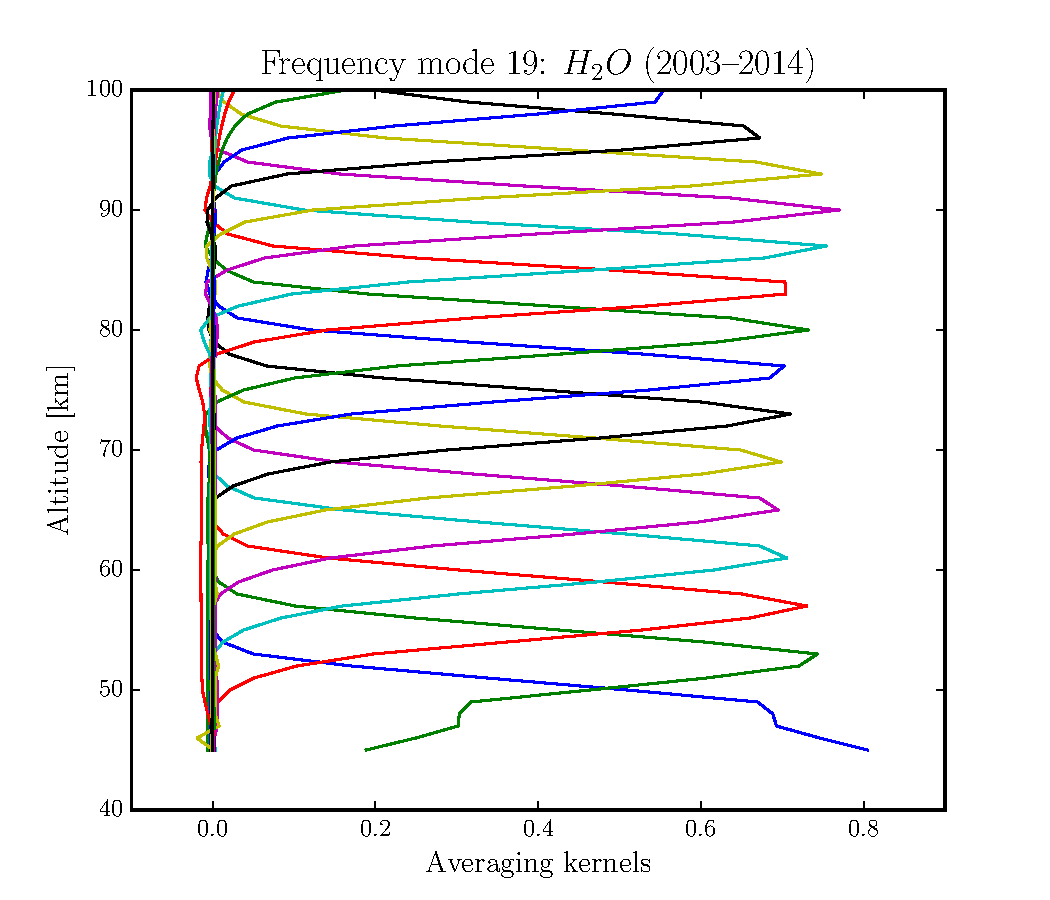
\includegraphics[width=\textwidth]{DDS_fm19_H2O_avk}
        \caption{median averaging kernels\newline~}
        \label{fig:fm19:H2O:avk}
    \end{subfigure}
    \caption{Measurement response and averaging kernels for \chem{H_2O}
    retrievals for \smr~v3 at different altitudes for frequency mode~19.}
    \label{fig:fm19:H2O:mr_avk}
\end{figure}


%%%%%%%%%%%%%%%
% Temperature %
%%%%%%%%%%%%%%%

\subsubsection{\chem{Temperature}}
\label{sec:fm19:comparison:temperature}
The retrievals for temperature have been compared with data from the MLS
instrument. Annual average differences to this instruments are shown in
Figure~\ref{fig:fm19:T:profiles}. In Figure~\ref{fig:fm13:T:scatter} individual
retrievals from MLS for the entire period are plotted against the retrievals
from the new and old versions of the \smr\ processing chain. The results show a
little or no improvement with the updated version of the processing. Whereas
with the previous version of the system, the temperature was under estimated
for lower temperatures and over estimated for higher, and a small systematic
under estimation of the temperature is now seen.
\TODO{reference Fig.~\ref{fig:fm19:T:mr_avk} in text!}

\begin{figure}[htpb]
    \centering
    \begin{subfigure}[b]{0.49\textwidth}
        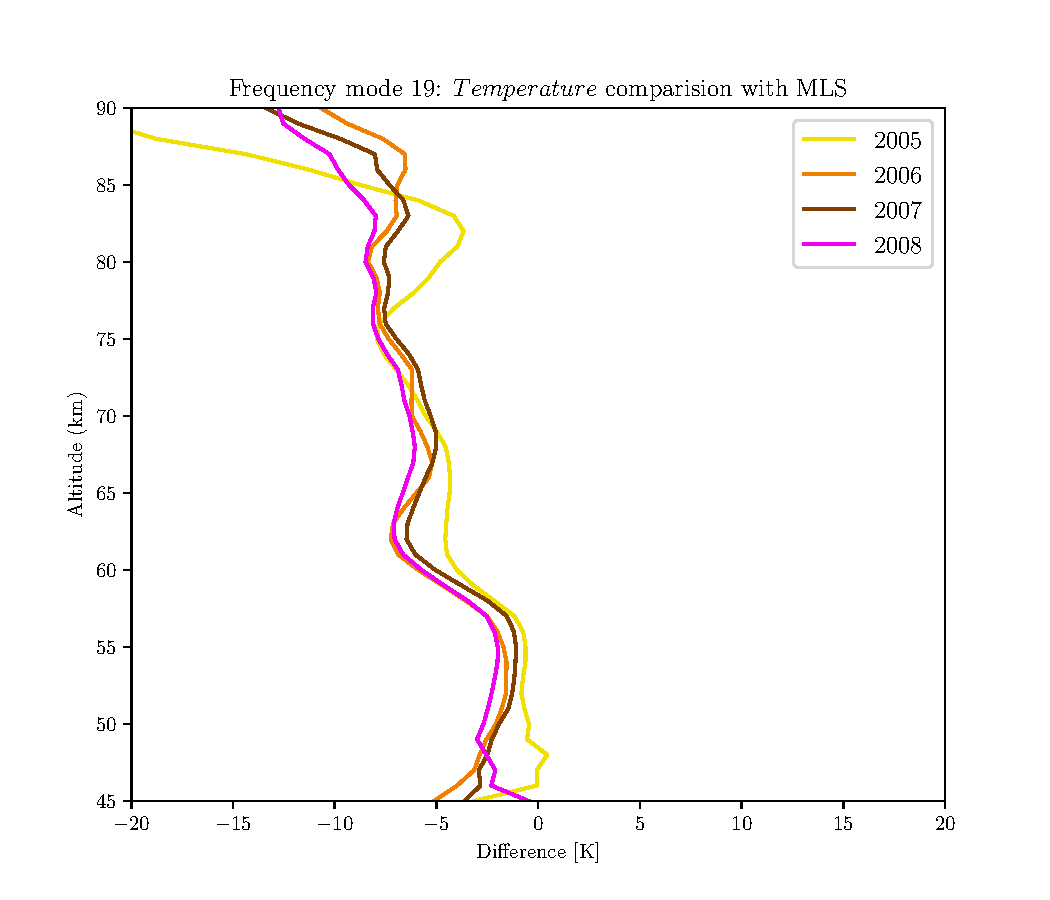
\includegraphics[width=\textwidth]{DDS_fm19_T_absdiff_mls}
        \caption{average difference to MLS}
        \label{fig:fm19:T:profiles:MLS}
    \end{subfigure}
    \caption{Average difference in K between retrievals of temperature from
    \smr~v3 and collocated measurements from MLS at different altitudes.}
    \label{fig:fm19:T:profiles}
\end{figure}

\begin{figure}[htpb]
    \centering
    \begin{subfigure}[b]{0.49\textwidth}
        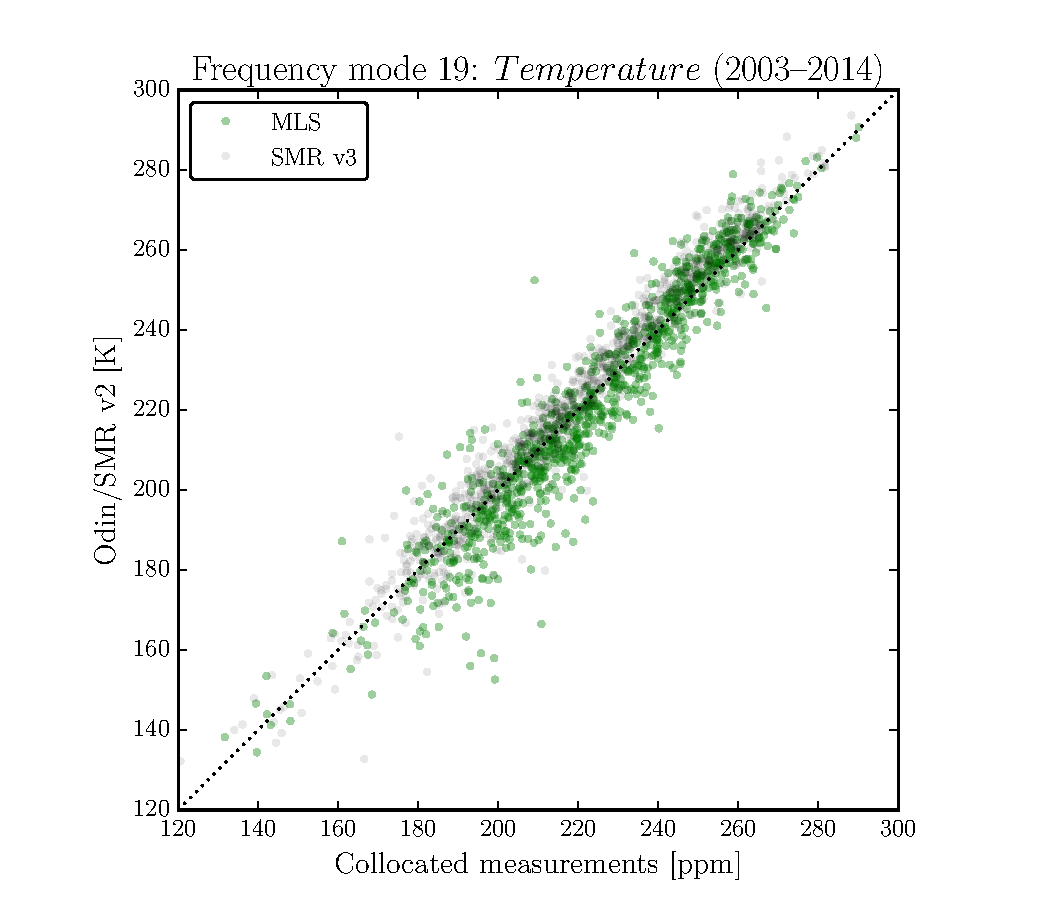
\includegraphics[width=\textwidth]{DDS_fm19_T_scatter_v2}
        \caption{correlation of collcated instruments with \smr~v2.X}
        \label{fig:fm19:T:scatter:v2}
    \end{subfigure}
    \,
    \begin{subfigure}[b]{0.49\textwidth}
        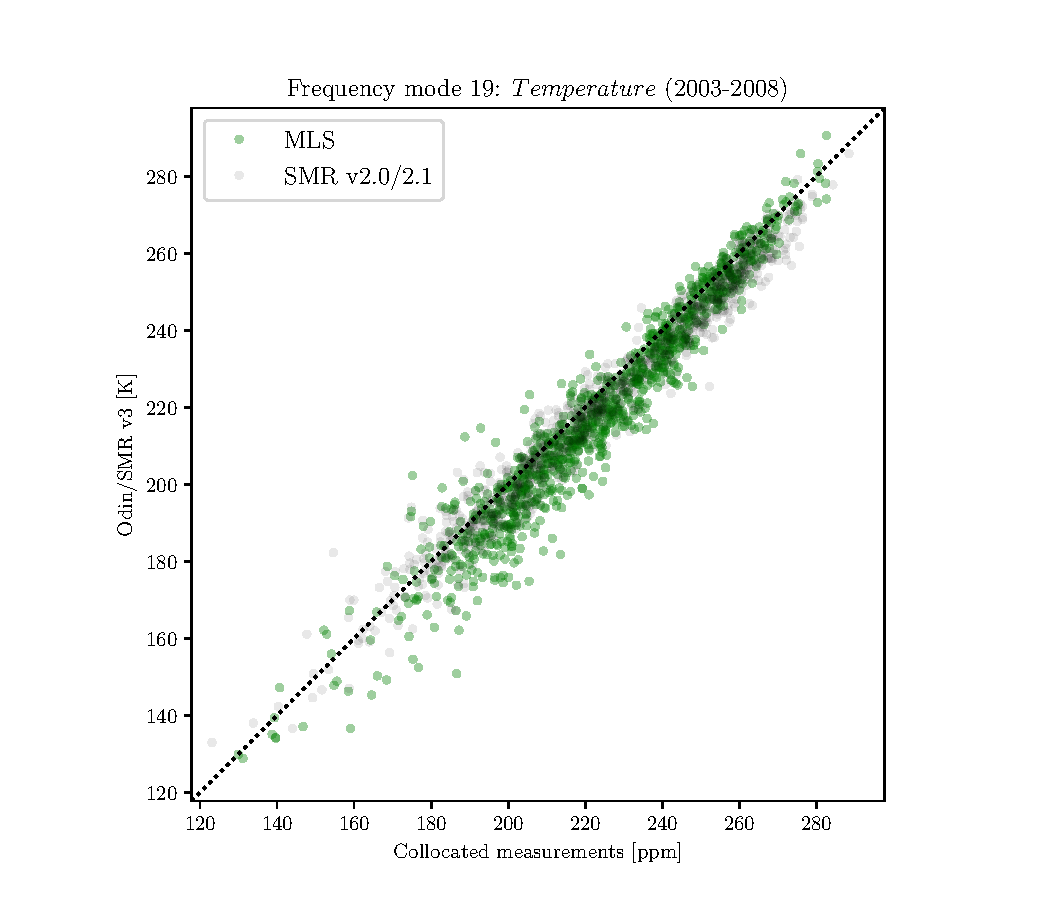
\includegraphics[width=\textwidth]{DDS_fm19_T_scatter_v3}
        \caption{correlation of collcated instruments with \smr~v3}
        \label{fig:fm19:T:scatter:v3}
    \end{subfigure}
    \caption{Correlation between retrievals of temperature using \smr\
    versions~2.X and~3 and collocated measurements from various instruments.}
    \label{fig:fm19:T:scatter}
\end{figure}

\begin{figure}[htpb]
    \centering
    \begin{subfigure}[b]{0.49\textwidth}
        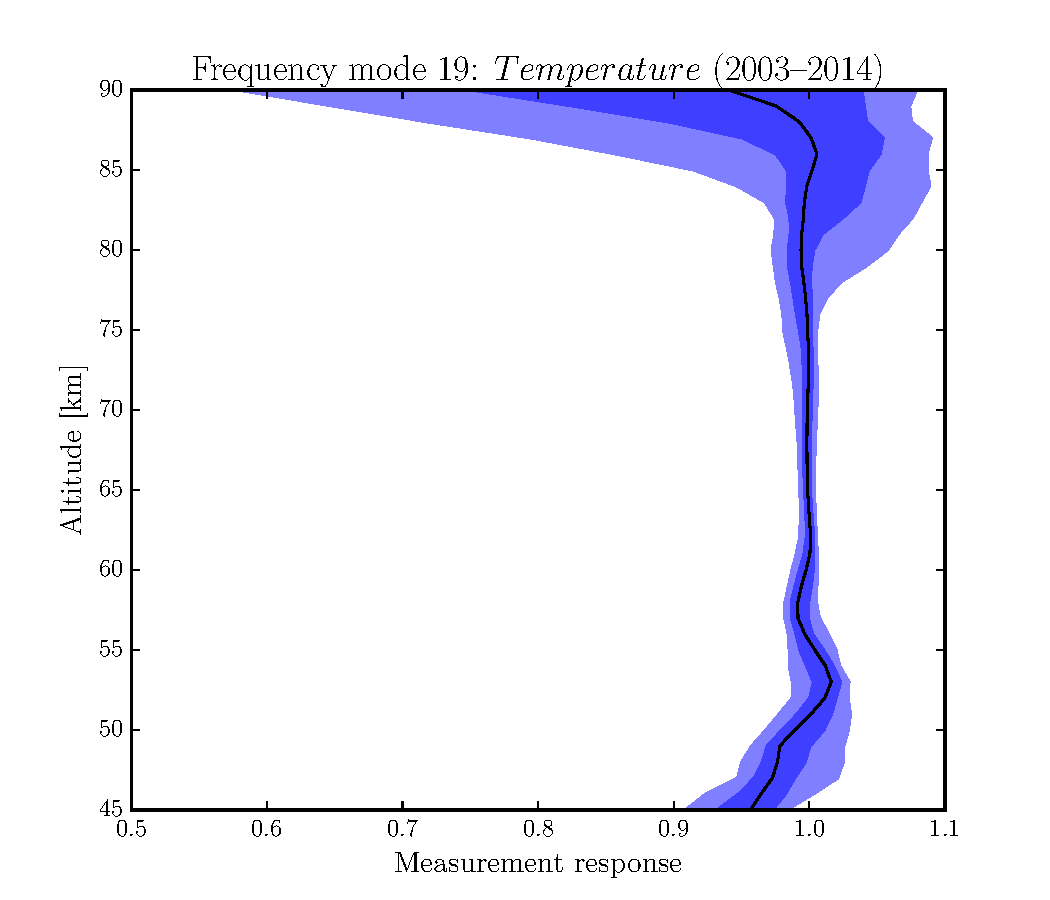
\includegraphics[width=\textwidth]{DDS_fm19_T_mr}
        \caption{median measurement response with $1\sigma$ and $2\sigma$
        percentiles}
        \label{fig:fm19:T:mr}
    \end{subfigure}
    \,
    \begin{subfigure}[b]{0.49\textwidth}
        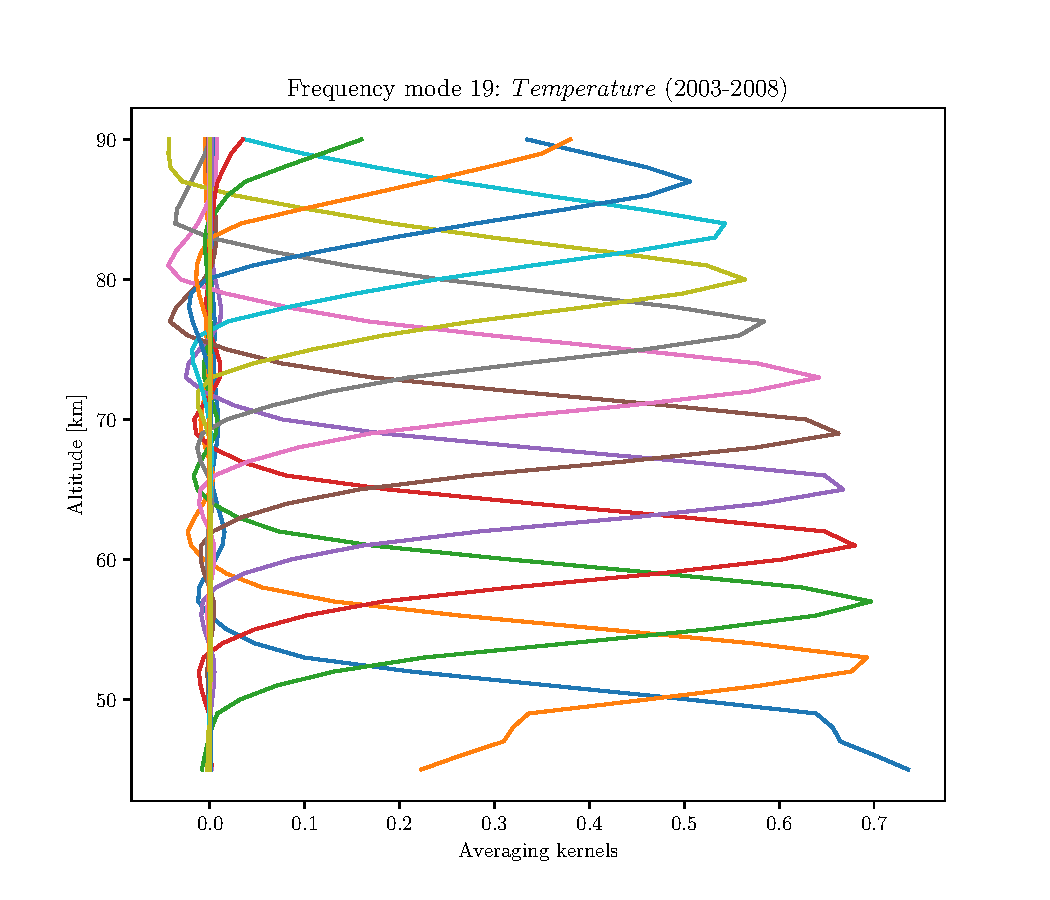
\includegraphics[width=\textwidth]{DDS_fm19_T_avk}
        \caption{median averaging kernels\newline~}
        \label{fig:fm19:T:avk}
    \end{subfigure}
    \caption{Measurement response and averaging kernels for temperature
    retrievals for \smr~v3 at different altitudes for frequency mode~19.}
    \label{fig:fm19:T:mr_avk}
\end{figure}


\subsection{Discussion}
\label{sec:fm19:discussion}
The Pearson correlation between the \smr\ retrievals and the other instruments
was calculated for the entire period for both versions of the processing chain.
The results are summarised in Table~\ref{tab:fm19:stats}, and show that the
new algorithm is a improvement compared to all the instruments for all species
used in this investigation. The improvement is considerable for both \chem{O_3}
and \chem{H_2O}.


\begin{table}[hbt]
\centering
\caption{Pearson correlation and fit parameters of the old and new \smr\
retrievals for frequency mode~19, compared with collocated data from other
instruments for the period 2003--2008.
}
\label{tab:fm19:stats}
\begin{tabular}{lllrrrr}
    \toprule
    \textbf{Species} & \textbf{Instrument} & \textbf{SMR} & \textbf{corr.} & \textbf{slope} & \textbf{intercept} & \textbf{$\left|\left<\right.\right.$res.$\left.\left.\right>\right|$} \\
    \midrule
    \chem{O3}   & MIPAS     & v3    & 0.779 & 0.733 & 0.088\,ppm    & 0.616\,ppm \\
                &           & v2.x  & 0.827 & 0.813 & -0.133\,ppm   & 0.599\,ppm \\
    \cline{2-7}
                & MLS       & v3    & 0.760 & 0.643 & 0.340\,ppm    & 0.627\,ppm \\
                &           & v2.x  & 0.793 & 0.688 & 0.168\,ppm    & 0.570\,ppm \\
    \cline{2-7}
                & OSIRIS    & v3    & 0.874 & 0.795 & 0.272\,ppm    & 0.327\,ppm \\
                &           & v2.x  & 0.873 & 0.880 & -0.143\,ppm   & 0.494\,ppm \\
    \cline{2-7}
                & SAGE~III  & v3    & 0.950 & 0.893 & 0.089\,ppm    & 0.270\,ppm \\
                &           & v2.x  & 0.924 & 0.861 & 0.005\,ppm    & 0.350\,ppm \\
    \midrule
    \chem{H_2O} & MIPAS     & v3    & 0.520 & 0.683 & -0.240\,ppm   & 2.885\,ppm \\
                &           & v2.x  & 0.478 & 0.688 & -0.016\,ppm   & 2.942\,ppm \\
    \cline{2-7}
                & MLS       & v3    & 0.899 & 0.758 & -0.177\,ppm   & 1.774\,ppm \\
                &           & v2.x  & 0.878 & 0.835 & -0.244\,ppm   & 1.685\,ppm \\
    \midrule
    Temp.       & MLS       & v3    & 0.964 & 1.041 & -14.848\,K    & 10.217\,K \\
                &           & v2.x  & 0.964 & 1.084 & -20.553\,K    &  8.423\,K \\
    \bottomrule
\end{tabular}
\end{table}

\subsection{Conclusions}
\label{sec:fm19:conclusions}
\TODO{Recommended usage: which species, which periods}
Based on the discussion above, retrievals based on frequency mode~19 should be
used with caution for both \chem{O_3} and \chem{H_2O}, but can be used with
confidence for temperature retrievals.
